\documentclass[12pt]{article}
\usepackage{german}
\usepackage{todonotes}
\usepackage{tikz}
\usepackage[utf8]{inputenc}
\usepackage{adjustbox}
\usepackage{graphicx}
\usepackage{afterpage}
\usepackage{listings}
\usepackage{float}
\usepackage[headsepline]{scrpage2}
\pagestyle{scrheadings}
\clearscrheadfoot
\graphicspath{{./images/}}

\lstset{language=Python}

\begin{document}

\ohead{Erianet}
\ihead{Florian Schwarcz \& Erik Mayrhofer}
\ofoot{\pagemark}

%\listoftodos
\tableofcontents
\newpage

\part{Erianet}
\section{Einleitung}
\subsection{Name}
Das Erianet ist eine mit Python entwickelte Software, die
durch ein neurales Netzwerk f"ahig ist,
Personen anhand ihrer Gesichter unterscheiden.
Es wurde von Mayrhofer Erik und Schwarcz Florian
entwickelt und durch Kombination beider Vornamen und {\glqq}neural net{\grqq}
auf seinen Namen getauft.
\subsection{Hintergrund}
Im Rahmen des Schulunterrichts im Fach {\glqq}Systemplanung und Projektentwicklung{\grqq}
war es die Aufgabe des Projektteams, eine zur Gesichtserkennung
f"ahige Software zu entwickeln.
%\todo{Welche Technologien}
Bei der Entwicklung bediente man sich einiger Python-Libraries.
So wurde OpenCV als Gesichtsdetektor eingesetzt und mit Keras das neurale
Netz erstellt und trainiert.
\subsection{Verwendete Ressourcen}
Zum Trainieren des Modells wurden vorgefertigte Sammlungen f"ur genau diesen
Zweck auf dem Internet verwendet. Einige davon waren die {\glqq}Labelled Faces in the Wild{\grqq},
{\glqq}AT\&T Faces{\grqq} und {\glqq}YouTube face database{\grqq}. Es wurden
auch selbst Bilder mit einem dazu erstellten Programm geschossen und zum Training verwendet.
\newpage
\section{Architektur}
\afterpage{\clearpage}
\begin{figure}[H]
    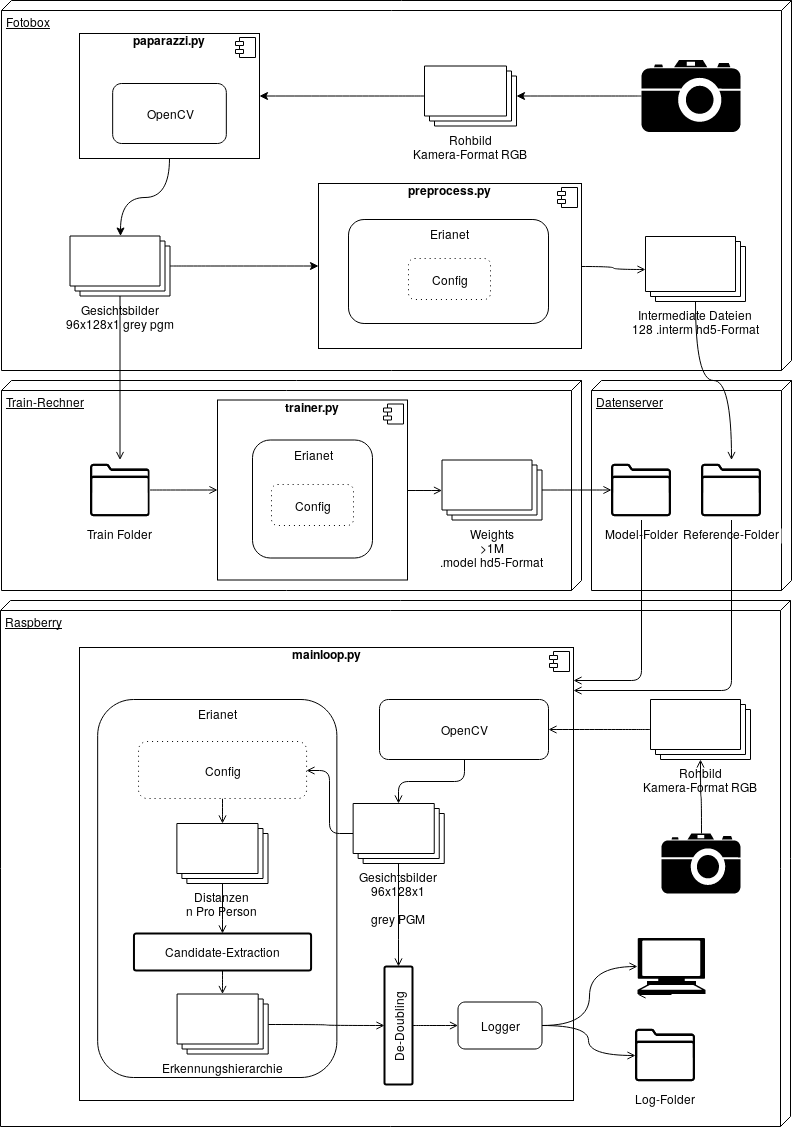
\includegraphics[height=0.9\textheight]{Architektur}
    \caption{Architektur}
\end{figure}

\subsection{Fotobox}
Die Fotobox ist ein kleiner Rechner,
mit dessen Hilfe Referenzbilder aufgenommen werden
k"onnen.
\paragraph{paparazzi.py}
greift den Kamera-Feed einer Webcam ab und nutzt
OpenCVs Haar-Classifier dazu, ein erkanntes Gesicht 
herauszuschneiden. Dieses wird dann in unser verwendetes
Format umgewandelt.
\paragraph{preprozess.py}
nimmt die vorher aufgenommenen Bilder und l"asst sie einmal 
durch einen Fu{\ss} des Erianet laufen. Dadurch
werden sie in die interne Repr"asentation des neuralen Netzes 
umgewandelt und als sogenannte intermediate-Datei gespeichert.
Dieser Schritt spart extrem viel Rechenzeit, da sonst
jedes einzelne Bild zur Laufzeit wieder und wieder 
umgewandelt werden m"usste.
\subsection{Train-Rechner}
Der Train-Rechner ist ein leistungsf"ahiger Rechner, welcher nur selten
ben"otigt wird. Damit das neurale Netz f"ahig wird, Gesichter verl"asslich
zu unterscheiden, muss man es trainieren. Das hei{\ss}t, man muss ihm viele
Daten geben, mit deren Hilfe es lernt, die vorgegebene Aufgabe zu erf"ullen.
\paragraph{Train Folder} Am Train-Rechner m"ussen die rohen
Bilder vorhanden sein, welche vorher aufgenommen wurden.
Diese Bilder m"ussen nicht zwingend Bilder von Menschen sein,
die man sp"ater erkennen m"ochte, sondern eine m"oglichst diverse
Menge an unterschiedlichen Bildern von Gesichtern. Um gute Ergebnisse
zu erzielen, rechnen wir damit, eine ungef"ahre Menge von insgesamt
10.000 Bildern von mindestens 500 Personen zu ben"otigen.
\paragraph{trainer.py}
Der Trainer nutzt die Referenzdaten aus dem Train Folder 
um die weights des neuralen Netzes zu ermitteln und diese
als trainiertes Modell zu speichern.
\subsection{Hauptrechner}
Am Hauptrechner w"urde die finale Gesichtserkennung stattfinden.
Dazu sind ein trainiertes Modell und die intermediate-Daten vonn"oten.
\paragraph{mainloop.py}
Die Mainloop ist das Hauptprogramm, das mithilfe des Erianet und einer Kamera
die aufgenommenen Gesichter erkennt und mitloggt.
\paragraph{Erianet}
Das Erianet im Mainloop wandelt ein aufgenommenes Gesichtsbild in
das Intermediate-Format um und vergleicht dieses "uber die 
euklid'sche Distanz mit den Referenzbildern aus dem Reference-Folder.
F"ur jede Referenzklasse wird dann die durchschnittliche Distanz
ermittelt und nach dieser werden die Klassen geordnet und als
Kandidaten wieder zur"uckgegeben.
\paragraph{Log-Folder}
Im Log-Verzeichnis wird in einer Textdatei jede Erkennung mitprotokolliert.
Sowohl die Zeit der Erkennung als auch der Name werden gespeichert und zu
jedem Eintritt wird das Bild der Person in den Pictures-Ordner gespeichert
und nach dem Logeintrag benannt.
\subsection{Formate}
\paragraph{Kamerarohbilder}
d"urfen so gro{\ss} sein wie die Kamera sie liefert und m"ussen RGB sein.
\paragraph{Gesichtsbilder}
sind 128 Pixel hoch und 96 Pixel breit und sollten in Greyscale 
sein.
\paragraph{Intermediate}
sind im HDF5-Format gespeichert und 128 floats lang.
\paragraph{Weights}
werden von Keras gespeichert, sind im HDF5-Format. 

\pagebreak
\section{Neurales Netz}
Als erianet.py wird in dieser Software eine Wrapper-Klasse f"ur 
Keras bezeichnet. Diese Klasse repr"asentiert eine Instanz des 
Erianet und bietet verschiedene Methoden an, welche die 
Bedienung um einiges einfacher machen. Der durchschnittliche
Lebenszyklus eines Erianet sieht folgenderma{\ss}n aus:
\begin{lstlisting}[frame=single]
net = Erianet("model.name", config=VGG19ish)

names = net.predict(image, reference_set)

for name in names:
    print(PredictResult.name(name), 
    PredictResult.difference(name))
\end{lstlisting}
In der Config sind die eigentlichen Layer des Neuralen Netzes definiert.
\subsection{Aufbau}
Das Erianet baut auf einem sogenannten {\glqq}Siamesischen Netzwerk{\grqq} auf.
Ein siamesisches Netzwerk zeichent sich dadurch aus, dass es zwei
{\glqq}F"u{\ss}e{\grqq} gibt, welche aus dem exakt gleichen Convolutional-Netzwerk 
bestehen und sich die weights teilen. Ein Bild wird durch den
einen Fu{\ss} geschickt, das andere Bild durch den anderen Fu{\ss}.
Ein Fu{\ss}netzwerk gibt jeweils einen Vektor (Intermediate-Repr"asentation)
zur"uck und zwischen diesen Vektoren wird dann die euklid'sche Distanz
gebildet, um festzustellen, wie "ahnlich die beiden Bilder sind.
\paragraph{Fu{\ss}netzwerk}
Das Fu{\ss}netzwerk ist meist ein Deep-Convolutional-Neural-Network, was hei{\ss}t,
dass viele Schichten von Convolutional-Layern und Pooling-Layern genutzt werden.
Der vielversprechendste Ansatz ist ein VGG19-Netzwerk.
\subsection{Training}
Das Training eines Siamesischen Netzwerks ist supervised. Das hei{\ss}t, dass
dem Netzwerk zwei Bilder gezeigt werden und je nachdem, ob die beiden Bilder
von derselben Person oder von unterschiedlichen Personen stammen, wird dann 
versucht die Distanz zwischen den Intermediate-Vektoren m"oglichst hoch bzw. 
niedrig zu halten.

\part{Facepong}
\section{Einleitung}
\subsection{Hintergrund}
F"ur den Tag der offenen T"ur an der HTL Leonding wurde dem Projektteam
aufgetragen, mithilfe ihrer gesammelten Erfahrung im Bereich Gesichtsdetektion
ein kleines Programm zu entwickeln, welches man den Besuchern Vorstellen kann.
Dabei kam die Idee auf, ein Spiel zu programmieren, bei dem man mit seinem Gesicht
gegen einen anderen Spieler das klassische Spiel {\glqq}Pong{\grqq} spielen kann.
\subsection{Verwendete Libraries}
Zus"atzlich zu OpenCV f"ur die Gesichtsdetektion wurden in diesem Teil des Projektes
die Libraries PyMunk f"ur realistische Physiksimulation und PyGame f"ur einfache Bildausgabe
herangezogen.
\section{Aufbau und Spielweise}
Zum Spielen braucht man eine Kamera und einen Monitor bzw. Beamer. Die Kamera
wird m"oglichst mittig entweder unter oder "uber der Bildausgabe aufgestellt und angeschlossen.
Anschlie{\ss}end wird das Programm gestartet und es kann gespielt werden.
Betreten die beiden Spieler ihren Bereich links und rechts vor der Kamera,
startet das Spiel automatisch. Der Ball kann nun mit dem Kopf angesto{\ss}en werden
und muss das Tor des Gegners ber"uhren. Zu beachten ist hierbei, dass
das Gesicht jederzeit gerade zur Kamera gerichtet sein muss, damit es erkannt werden kann.
\section{Probleme und Zukunftspl"ane}
\subsection{Gesichtserkennung}
Wie bereits erw"ahnt muss man den Kopf zu jeder Zeit gerade in Richtung
der Kamera halten. Dadurch wird bei zu gro{\ss}er Neigung durch nach unten oder zur
Seite blicken das Spiel angehalten, da kein Gesicht erkannt wird.
Die Behebung des oben genannten Problems k"onnte durch Einsatz besserer
Modelle unter R"ucksichtnahme auf die Performance m"oglich sein.
\subsection{Aufl"osung und Performance}
Das Spiel l"auft aktuell einer Aufl"osung von 480p und verlangsamt sich beim Upgrade auf 1080p
auf unter 10 Bilder pro Sekunde, was auf das inperformante Modell zur
Gesichtsdetektion zur"uckzuf"uhren ist. F"ur den jetzigen Einsatz mit
Beamer und Kamera sind 480p jedoch ausreichend.
\section{Architektur}
\paragraph{PongGame}
k"ummert sich um die Hauptloop, welche den aktuellen Gamestate aufruft, dann die 
Grafik rendert und schlussendlich die Keyboard-Events bearbeitet.
Der Hauptloop holt sich auch die Bilder der Kamera und versucht die Framerate 
stabil zu halten.
\paragraph{pongFaceDetector}
k"ummert sich darum, aus dem mitgegeben Bild erkannte Gesichter herauszukratzen.
Der Haar-Classifier aus OpenCV sucht sich die Gesichter heraus und danach wird
der wahrscheinlichste Kandidat genommen und als finales Gesicht zur"uckgegeben.
\paragraph{pongConfig}
behinaltet eine Reihe von Datenklassen, welche grunds"atzliche Variablen beherbergen,
damit man FacePong schnell und effizient an die Umgebung anpassen kann.
\paragraph{pongPhysics}
bildet eine Wrapperklasse um PyMunk, und k"ummert sich darum, dass die Spielobjekte richtig
positioniert werden. Eigene Objekte werden gebildet aus: Gesichtern, R"andern des Spielfelds und 
dem Ball. In dieser Klasse wird auch erkannt, ob der Ball in ein Tor oder aus dem Spielfeld
geflogen ist.
\paragraph{pongRenderer}
sorgt daf"ur dass das Kamerabild richtig dargestellt wird. Die eigentlichen Spielobjekte
werden vom Gamestate gezeichnet, pongRenderer behinhaltet aber ein paar Hilfsmethoden,
um z.B Linien, Kreise o."a. zu zeichnen. Manche Objekte k"onnen in zwei Ebenen gezeichnet
werden (draw\_in\_front), damit z.B. Text alle anderen Spielobjekte "uberdeckt.
\paragraph{GameState}
werden im selben File wie pongGame geschrieben und beinhalten jeweils eine Methode zum 
rendern und zum updaten der Spiellogik. Um den GameState zu wechseln wird die Methode
game.change\_state\_to(newState) aufgerufen.


\end{document}